\section{Octavo \textit{sprint} de producción}
En este \textit{sprint} se implementa en código la funcionalidad de todos los 
elementos controladores del juego y sus auxiliares, exceptuando a los 
controladores de los niveles ya que éstos se desarrollarán en el décimo 
\textit{sprint} dado que se requieren los niveles terminados para comprobar su 
funcionalidad.

\subsection{Controlador de Audio}
Este controlador es el encargado de gestionar los efectos de sonido del 
juego. Logra su funcionamiento con ayuda de la clase controladora 
\textit{AudioCtrl} y de la clase auxiliar \textit{PlayerAudio}. 
\\
\par
La clase \textit{PlayerAudio} está compuesta de los atributos del tipo 
\textit{AudioClip}. Por convención los archivos de audio que \textit{Unity} 
soporta pueden ser del tipo \textit{MP3}, \textit{OGG}, \textit{WAV}, entre 
otros, en relación a tamaño del archivo y calidad de audio se opta por utilizar 
los archivos de tipo \textit{OGG}. Para la importación de los archivos de audio 
se elige la configuración que se muestra en la figura \ref{fig:AudioClipConfi}, 
ya que ésta se disminuye el tiempo de carga de los audios y el espacio en 
memoria de almacenamiento que utilizan dentro de la aplicación. 
\textit{PlayerAudio} contiene cinco pistas de audio correspondientes a los 
efectos de sonido cuando: 
	\begin{itemize}
		\item El jugador hace contacto con un objeto coleccionable, como una 
		llave o un \textit{xoloitzcuintle}.
		\item El jugador hace contacto con un ítem.
		\item El jugador dispara \textit{tonalli}.
		\item Un enemigo es destruido.
		\item El jugador muere.
	\end{itemize}	 

\textit{PlayerAudio} se vale de la serialización para su funcionamiento(ver 
figura \ref{fig:PlayerAudio}), esta clase funge como un organizador de elementos 
para su visualización en el \textit{GameInspector}, como se ve en la figura 
\ref{fig:PlayerAudioConf}.   

	\begin{figure}[h]
		\centering
		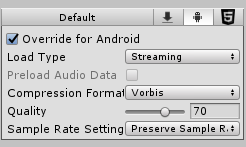
\includegraphics[height=0.15 \textheight]{03TrabajoRealizado/imagenes/playerAudioConfig.png}
		\caption{Configuración de la importación de los archivos de audio.}
		\label{fig:AudioClipConfi}
	\end{figure}

	\begin{figure}[h]
		\centering
		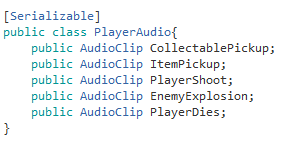
\includegraphics[height=0.15 \textheight]{03TrabajoRealizado/imagenes/playerAudio.png}
		\caption{Serialización de la clase \textit{PlayerAudio}}
		\label{fig:PlayerAudio}
	\end{figure}


	\begin{figure}[h]
		\centering
		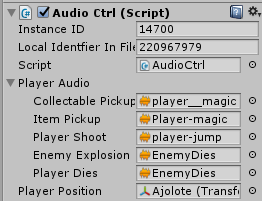
\includegraphics[height=0.1 \textheight]{03TrabajoRealizado/imagenes/audioCtrlGameInsp.png}
		\caption{Atributos organizados en el \textit{GameInspector} gracias a la serialización de la clase \textit{PlayerAudio}.}
		\label{fig:PlayerAudioConf}
	\end{figure}

Por su parte la clase \textit{AudioCtrl} tiene como atributos la clase 
\textit{PlayerAudio}, un vector de tres dimensiones para la posición del 
personaje que mande a llamar los métodos que invocan los audios y una instancia 
de la misma clase \textit{PlayerAudio} para la perseverancia de datos. Los 
métodos que contiene la clase son para invocar determinado audio, para esa 
funcionalidad se utiliza el método \textit{PlayClipAtPoint}, el cual necesita 
como atributos un objeto de tipo \textit{AudioClip} y un vector de tres 
dimensiones. Cada método que invoca un efecto de audio es mandado a llamar en la 
parte del código que implementa dicha funcionalidad, por ejemplo en el método 
\textit{SetHealth} del la clase \textit{Enemy} se agrega la linea de código que 
invoca el audio para la destrucción de un Enemigo en donde se maneja la muerte 
del enemigo. En la figura se pueden ver los atributos y los métodos de la clase 
\textit{AudioCtrl}.  

	\begin{figure}[h]
		\centering
		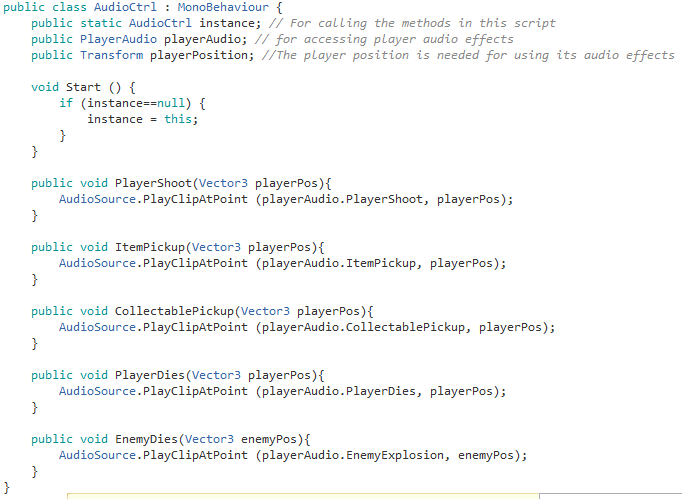
\includegraphics[height=0.3 \textheight]{03TrabajoRealizado/imagenes/audioCtrl.png}
		\caption{Atributos y métodos de la clase \textit{AudioCtrl}.}
		\label{fig:AudioCrl}
	\end{figure}
Para la musica de fondo de los niveles se tomaron fragmentos de la banda sonora 
de juegos como Final Fantasy XV, Final Fantasy XV royal edition, Kingdom Hearts 2 
y Klonoa 2: Lunatea's Veil; por lo que para la comercialización del juego se deben 
de modificar estos archivos de audio por original o de licencia libre.
\subsection{Controlador de Diálogos}\label{ControladorDialogo}
Este controlador se emplea en la cinemáticas del juego.El controlador de 
Diálogos se vale de cuatro clases para su funcionamiento: 
\textit{Dialogue}, \textit{Dialogues}, \textit{DialogueFile} y 
\textit{DialogueCtrl}. 
\\
\par
Las clases \textit{Dialogue} y \textit{Dialogues}, son clases de tipo auxiliar. Ambas clases son serializadas y el objetivo de ellas es el de organizar la información en el \textit{GameInspector}. La clase \textit{Dialogue} tiene como atributos un \textit{string} para almacenar el nombre del personaje al que pertenece el dialogo y una lista de tipo \textit{string} para los diálogos. Por su parte la clase \textit{Dialogues} tiene como atributo una lista de tipo \textit{Dialogue}. El objetivo de la clase \textit{Dialogues} es la de almacenar todos los diálogos de la cinemática. En la figura \ref{fig:Dialogues} se puede ver la definición de las clases \textit{Dialogue} y \textit{Dialogues}.
\\
\par
La clase \textit{DialogueFile} se encarga de la gestión de los diálogos, al contenerlos y activar la visualización de los mismos por medio de la clase \textit{DialogueCtrl}. 
\\
\par 
La clase \textit{DialogueCtrl} se encarga de la visualización de los diálogos 
dentro de la escena. Por tal motivo parte de sus atributos son 
\textit{GameObjects} del tipo \textit{Text} de la \textit{UI}. La clase 
\textit{DialogueCtrl} visualiza los diálogos tomando el contenido de la clase 
\textit{Dialogue} y extrayendo elemento por elemento. De cada elemento extraído 
se obtiene su lista de diálogos y se almacena esta lista en un \textit{Queue} y 
se muestra en pantalla cada dialogo. La transición entre diálogos se hace si el 
jugador oprime el botón de salto, ver figura \ref{fig:NextDialogueBottom}. Una 
vez que el controlador ha mostrado todos los diálogos de un elemento. Los 
diálogos se visualizan por medio de una animación que nuestra carácter por 
carácter, en la figura \ref{fig:DialoguesCtrl} se muestra el método encargado de 
mostrar esta animación.   

	\begin{figure}[h]
		\centering
		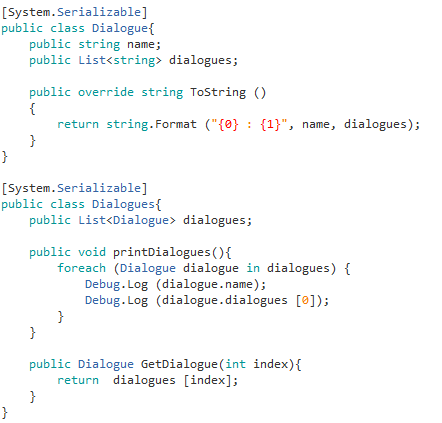
\includegraphics[height=0.3 \textheight]{03TrabajoRealizado/imagenes/dialogueFile.png}
		\caption{Serialización de las clases \textit{Dialogue} y \textit{Dialogues}.}
		\label{fig:Dialogues}
	\end{figure}

	\begin{figure}[h]
		\centering
		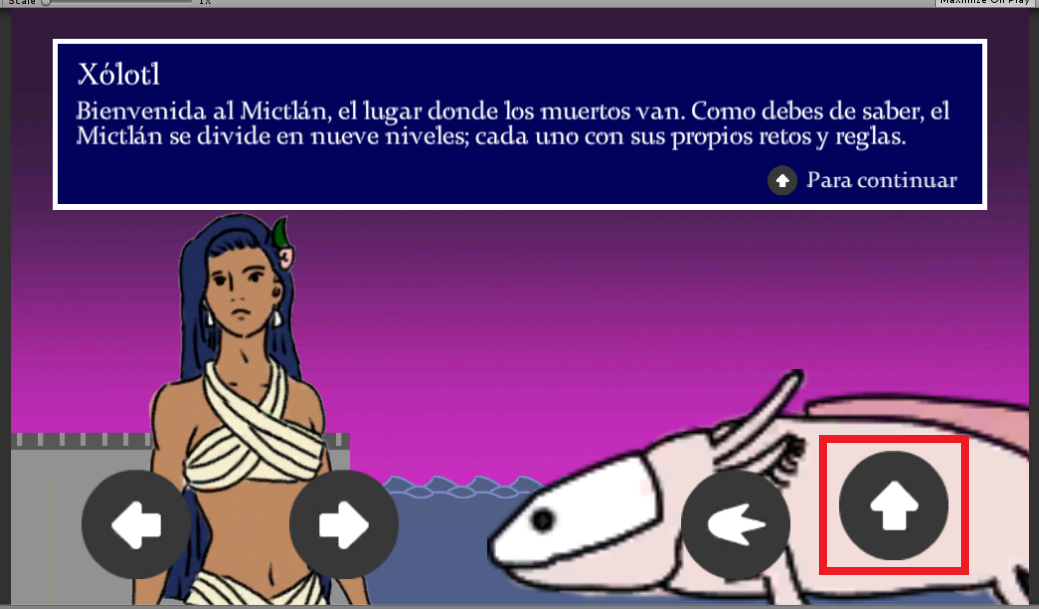
\includegraphics[height=0.2 \textheight]{03TrabajoRealizado/imagenes/DialogueOnScreen.png}
		\caption{La transición entre diálogos se hace si el jugador oprime el 
		botón de salto, este botón es el que se encuentra encerrado en rojo.}
		\label{fig:NextDialogueBottom}
	\end{figure}

	\begin{figure}[h]
		\centering
		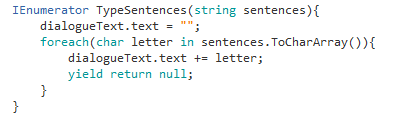
\includegraphics[height=0.15 \textheight]{03TrabajoRealizado/imagenes/dialogueController02.png}
		\caption{El método \textit{TypeSentences} es el encargado de animar el texto de los diálogos al mostrarlos en pantalla}
		\label{fig:DialoguesCtrl}
	\end{figure}

\subsection{Controlador de los datos del juego}
El controlador de datos del juego es el encargado de gestionar los datos 
relacionados al progreso del jugador, es decir los niveles desbloqueados, la 
cantidad de vida, la cantidad de \textit{tonalli}, el marcador y la cantidad de 
daño que hacen los ataques del jugador. Para su funcionamiento, este controlador 
se vale de las clases \textit{GameData} y \textit{GameDataCtrl}.
\\
\par
La clase \textit{GameData}, es una clase de tipo auxiliar y su función es la de 
serializar los datos que se van a almacenar en el archivo de los datos del 
juego, ver figura \ref{fig:GameData}. Por su naturaleza esta clase solo contiene 
la definicion de los atributos y sus \textit{getters} y \textit{setters}. 
\textit{Unity} maneja un tipo de archivo binario que permite la codificación de 
los datos para evitar que estos sean modificados por el jugador.
\\
\par
La clase \textit{GameDataCtrl} es la encargada de gestionar la creación del 
archivo, el cargado de la información y de salvar el progreso del jugador. Esta 
clase se debe de encontrar presente en todas las escenas del juego, ya que de 
los datos que ésta obtiene se inicializan los valores de la clase 
\textit{Player} y se verifican de los niveles disponibles. \textit{Unity} 
destruye todos los datos de una escena una vez que sale de ésta y crea una 
nueva, por lo que en cada escena se debería crear una instancia de la clase 
\textit{GameDataCrl}. Para evitar que se desperdicien recursos en el proceso de 
creación y destrucción de las instancias de la clase \textit{GameDataCrl} se 
recurre al patrón de diseño\textbf{ \textit{Singleton}}. El patron de diseño 
\textit{Singleton} garantiza que exista solo una instancia de una clase, lo que 
para el caso particular de \textit{Unity} se traduce en persistencia de la 
información entre escenas. En la figura \ref{fig:GameDataCtrl} se puede observar 
como se logra el comportamiento de un \textit{singleton} al agregar el método 
\textit{DontDestroyOnLoad}. El uso de un \textit{sigleton} hace que se tenga una 
configuración especial para el \textit{GameObject} que contenga a esta clase y 
garantizar que se tenga una única instancia. El \textit{GameObject} que contenga 
a la clase \textit{GameDataCtrl} debe de estar únicamente en la escena del menú 
principal y no debe de encontrarse en ninguna otra. Para probar el 
funcionamiento de los niveles del juego se puede tener tener un 
\textit{GameObject} que contenga a la clase \textit{GameDataCtrl} en dichas 
escenas pero es importante que cuando se construya la \textit{apk} del juego, 
todos estos \textit{GameObjects} se desactiven o se eliminen para evitar crear 
conflictos por múltiples instancias de la clase \textit{GameDataCtrl}.  

	\begin{figure}[h]
		\centering
		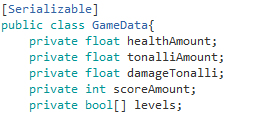
\includegraphics[height=0.15 \textheight]{03TrabajoRealizado/imagenes/GameData.png}
		\caption{Los atributos de la clase \textit{GameData} corresponden a los 
		datos que se guardaran en el archivo del progreso del juego por lo que 
		estos atributos se encuentran serializados}
		\label{fig:GameData}
	\end{figure}   
	
	\begin{figure}[h]
		\centering
		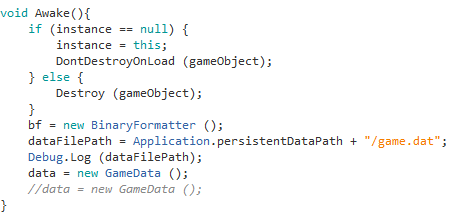
\includegraphics[height=0.2 \textheight]{03TrabajoRealizado/imagenes/gameDataCtrl.png}
		\caption{Inicialización de la clase \textit{GameDataCtrl} para 
		garantizar el patrón de diseño \textit{Singleton}.}
		\label{fig:GameDataCtrl}
	\end{figure}

\subsection{Controlador de fin de la partida}
El controlador de fin de partida funciona a partir de la clase 
\textit{GameOverCtrl} y de un \textit{GameObject} de tipo \textit{Panel}. La 
logica detras este controlador es la siguiente, en el \textit{Panel} se 
contienen los botones que tienen la funcionalidad de la interfaz que se muestra 
cuando el jugador ha muerto dentro del juego, ver figura 
\ref{fig:GameOverInterfaz}. La interfaz de fin de partida esta compuesta de tres 
botones uno para reiniciar la partida, otro para volver al menú de selección de 
nivel y el tercero para salir de la aplicación. La clase \textit{GameOverCtrl} 
se encarga de la funcionalidad de los botones y de hacer aparecer el 
\textit{panel} cuando el jugador es derrotado. En la figura 
\ref{fig:GameOverCtrl} se pueden observar los métodos de la clase \textit{GameOverCtrl}. 

	\begin{figure}[h]
		\centering
		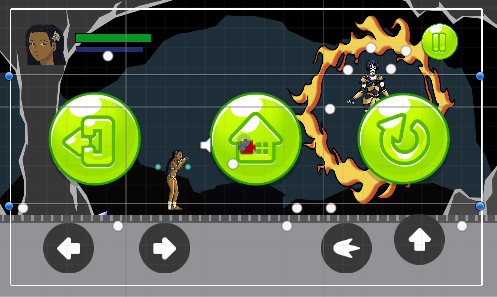
\includegraphics[height=0.2 \textheight]{03TrabajoRealizado/imagenes/GameOverPanel.png}
		\caption{Interfaz que aparece cuando el jugador ha muerto dentro del juego para indicar que ha perdido.}
		\label{fig:GameOverInterfaz}
	\end{figure} 
	
	\begin{figure}[h]
		\centering
		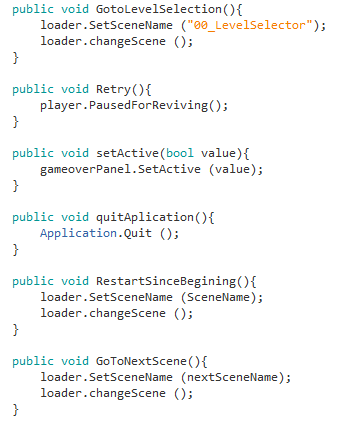
\includegraphics[height=0.2 \textheight]{03TrabajoRealizado/imagenes/GameOverCtrl.png}
		\caption{Métodos de la clase GameOverCtrl}
		\label{fig:GameOverCtrl}
	\end{figure} 

\subsection{Controlador de la barra de vida y de \textit{tonalli} del jugador}
Este controlador se encarga de actualizar gráficamente la cantidad de vida y 
\textit{tonalli} con la que cuenta el jugador. Para la funcionalidad de este 
controlador se implementa un \textit{Panel} \textit{GameObject} para que 
contenga las barras de vida y tonalli del jugador del jugador. Las barras de 
vida y de tonalli se crean usando \textit{UI GameObjects} de tipo 
\textit{Image}. Para la barra de vida se emplean tres \textit{UI GameObjects} de 
tipo \textit{Image}:  
	\begin{itemize}
		\item \textit{Health}: de color verde, que representa la cantidad de 
		vida del jugador.
		\item \textit{Damage}: De color rojo, representa la cantidad de daño que 
		recibe el jugador, es del mismo tamaño que \textit{Health}.
		\item \textit{BarHealth:} De color negra, es ligeramente de mayor tamaño 
		que las dos anteriores y funge como borde para la barra de vida. Ver figura  \ref{fig:HealthBar}.
	\end{itemize}
La actualización de la barra de vida se consigue redimensionando el tamaño de 
\textit{Health}, Unity cuenta con el método \textit{localScale} que permite 
ajustar la dimensión de un \textit{GameObject}. \textit{LocalScale} requiere 
como argumento un vector de dos dimensiones para indicarle si se hará un ajuste 
horizontal o vertical del objeto, este método toma el 1 como la máxima dimensión 
del objeto por lo que si se quisiera que el la barra de vida se redujera a la 
mitad, se tendría que enviar como argumento al método un vector de $(0.5, 1)$. 
Para el valor en $x$ de la escala a la que se va a redimensionar \textit{Health} 
basta con dividir la cantidad actual de vida entre la cantidad máxima, es decir 
$health/maxHealth$. Para actualizar la barra de tonalli se requiere del mismo 
método. La clase \textit{HealthBar} es la encargada de gestionar el 
redimensionamiento de las barras de vida y de tonalli. Sus métodos 
\textit{UpDateHealthBar} y \textit{UpDateTonallithBar} son llamados en la clase 
\textit{Player} en los métodos \textit{SetHealt} y \textit{SetTonalli}, métodos 
encargados de actualizar la cantidad de vida y de \textit{tonalli} 
respectivamente. 

	\begin{figure}[h]
		\centering
		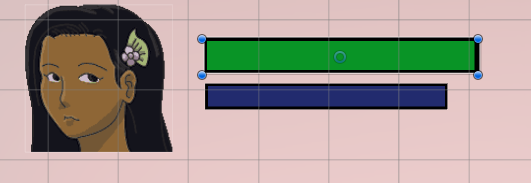
\includegraphics[height=0.1 \textheight]{03TrabajoRealizado/imagenes/attributesBar.png}
		\caption{Barras de vida y \textit{tonalli}.}
		\label{fig:HealthBar}
	\end{figure} 
	
\subsection{Controlador del panel de marcadores}
El controlador del panel de marcadores es el encargado de actualizar gráficamente cuantos objetos coleccionables ha juntado el jugador dentro de un nivel, ya sean llaves o \textit{xoloitzcuintles}, ver figura \ref{fig:HUB}. Para implementar la actualización gráfica de los marcadores ser crea un \textit{panel} \textit{GameObject} para contener los iconos de los objetos coleccionables y el texto que proporciona la información de los mismos. La clase \textit{HUBCtrl} es encargada de actualizar el texto referente a los marcadores; para tal funcion se vale de dos métodos:

	\begin{itemize}
		\item \textit{\textbf{UpDateDogScore:}}responsable de actualizar el conteo de \textit{xoloitzcuintles} y del poder de \textit{Xochitonal} en el segundo nivel.
		 \item \textit{\textbf{UpDateKeys:}} encargado de actualizar la cantidad de llaves colectadas en el cuarto nivel.
	\end{itemize}	 
	
	Estos métodos son mandados a llamar por la clase \textit{Player} en su método \textit{OnTriggerEnter2D}, ya que este es el que gestiona las reacciones del jugador y del juego ante las colisiones del jugador.

	\begin{figure}[h]
		\centering
		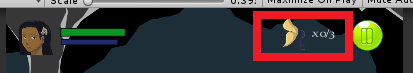
\includegraphics[height=0.05 \textheight]{03TrabajoRealizado/imagenes/HUB.png}
		\caption{Panel del marcador correspondiente al nivel 4.}
		\label{fig:HUB}
	\end{figure} 
	
\subsection{Controlador de pausa en el juego}
Este controlador permite pausar el nivel que se esta jugando al oprimir el botón 
de pausa que se encuentra en la esquina superior derecha de la pantalla, ver 
figura \ref{fig:PausedFuctionality}. Para implementar esta funcionalidad se 
agrega el botón de \textit{pausa} al panel de marcadores y se crea un nuevo 
panel parecido al de fin de partida con la diferencia que en lugar del botón de 
reintentar partida se pone el botón de quitar pausa del juego, ver figura 
\ref{fig:PausedFuctionality}. Dado que dos de los botones tienen la misma 
funcionalidad que el panel de fin de partida, los botones para salir de la 
aplicación y para ir al menu de selección de nivel toman la funcionalidad del 
\textit{GameOverCtrl}; mientras que el botón de pausa y de botón para quitar la 
pausa del juego toman su funcionalidad de la clase \textit{PauseCtrl}. La 
funcionalidad de \textit{PauseCtrl} se basa en el flujo del tiempo de la 
partida. \textit{Unity} permite controlar la velocidad de la partida con el 
atributo \textit{timeScale} de la clase \textit{Time}, donde el valor uno es el 
flujo normal del tiempo y cero es detener la partida. \textit{PauseCtrl} utiliza 
dos métodos en donde controla la velocidad del juego y desaparece o hace visible 
el panel de juego pausado; el primer método, llamado \textit{SetGamePaused}, es 
el encargado de hacer que la velocidad del juego sea igual a cero y de hacer 
aparecer el panel de juego pausado; el segundo método, llamado 
\textit{SetGameActive} regresa el juego a su flujo de tiempo habitual al 
asignarle un valor de uno a \textit{timeScale} y desactiva el panel de juego 
pausado. En la figura \ref{fig:pauseMethods} se pueden ver ambos métodos en 
código. 

\begin{figure}
  \centering
   \subfigure[Botón de pausa ubicado en la esquina superior izquierda.] {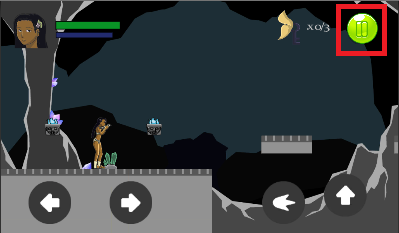
\includegraphics[width=0.3 \textwidth]{03TrabajoRealizado/imagenes/pauseBotton}}
   
 	\subfigure[Interfaz de partida pausada.] {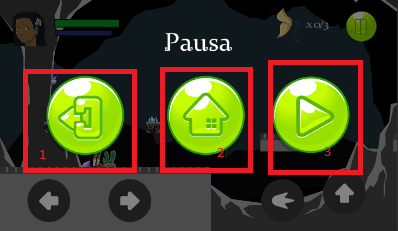
\includegraphics[width=0.3 \textwidth]{03TrabajoRealizado/imagenes/pauseInterface}}
 	

  \caption{Componentes en \textit{GameObject} para la funcionalidad de pausar 
  partida. La funcionalidad de los botones queda dada por : 1, Botón para salir 
  de la aplicación; 2, botón para volver al menú de selección de nivel; 3, botón 
  para quitar la pausa del juego. }
  \label{fig:PausedFuctionality}
\end{figure} 

\begin{figure}[h]
		\centering
		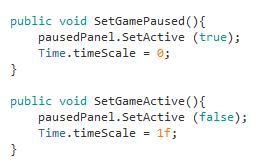
\includegraphics[height=0.2 \textheight]{03TrabajoRealizado/imagenes/Paused.png}
		\caption{La pausa se logra con los métodos \textit{SetGamePaused} y 
		\textit{SetGameActive} encargados de controlar el valor del atributo 
		\textit{timeScale} de la clase \textit{Time}.}
		\label{fig:pauseMethods}
	\end{figure} 
	
\subsection{Controlador de efectos especiales}
Este controlador muestra dos efectos especiales: una explosion cunado un enemigo o el jugador son derrotados y un destello cuando el jugador toca un ítem o un objeto colleccionable. Para generar el controlador se utilizan dos clases:

\begin{itemize}
	\item \textit{\textbf{SFX:}} Clase auxiliar que implementa la serialización para agrupar los \textit{assets} que generan los efectos, ver figura.
	\textit{\textbf{SFXCrl:}} Clase controladora encargada de instanciar los efectos dentro de la escena dado un vector de posición de tres dimensiones.
\end{itemize}

Como sucede con el controlador de efectos de sonido, los métodos que generan los efectos especiales de la clase \textit{SFXCtrl} son mandados a llamar dentro de otras clases como \textit{Player} o \textit{Enemy} cuando el jugador o el enemigo muere y el el gestor de colisiones de la clase \textit{Player}.

\subsection{Cierre del sprint}
Este \textit{sprint} se finaliza sin contratiempos y logrando el objetivo del 
mismo, que es generar los controladores comunes de los niveles. Por tal motivo, al 
finalizar el octavo \textit{sprit} se cuentan con los controladores y actores 
suficientes como para construir los niveles restantes. 
\\
\par
Para iniciar la construcción de los niveles se crea una escena base que contenga 
todos los controladores y al personaje jugable totalmente configurado con sus 
clases auxiliares, ver figura \ref{fig:EscenaBase}. Se decide crear esta escena 
para no invertir tiempo en la creación y configuración de los elementos comunes 
de los niveles. Con esta escena creada se dejan preparadas todas las herramientas 
para el siguiente \textit{sprint}.

\begin{figure}
  \centering
  
   \subfigure[Vista de la escena base del juego.] {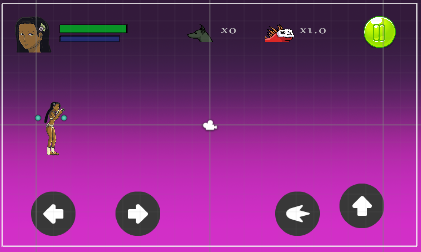
\includegraphics[width=0.3 \textwidth]{03TrabajoRealizado/imagenes/escena00}}
   
 	\subfigure[Vista de los objetos que contiene la escena base del juego desde la pestaña de jerarquía.] {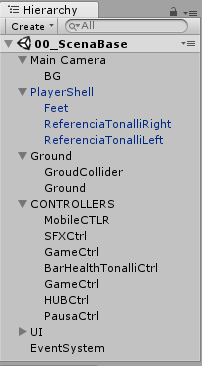
\includegraphics[width=0.15 \textwidth]{03TrabajoRealizado/imagenes/escena00Hierarchy}}
 	

  \caption{Vista de la escena base que contiene todos los controladores y al 
  personaje jugable configurado.}
  \label{fig:EscenaBase}
\end{figure} 

